\documentclass[letterpaper, 11pt]{article}

% ==============================================================================
% CARGA DE PAQUETES Y CONFIGURACIONES GLOBALES
% ==============================================================================
\usepackage{graphicx}
\usepackage{geometry}
\geometry{
    letterpaper,
    top = 2.5cm,
    bottom = 2.5cm,
    left = 2cm,
    right = 2cm,
    headheight = 14pt
}
\usepackage[utf8]{inputenc}
\usepackage[spanish]{babel} % Renombra en automático los elementos a español
\usepackage{float}  % Etiqueta 'H' (mayus) en figuras (imágenes)
\usepackage{array}  % Padding en tablas
\usepackage{url}    % Etiqueta url en .bib
\usepackage{booktabs}   % Manejo de caudros (tablas)
\usepackage[T1]{fontenc}    % Codificación de fuentes
\usepackage{csquotes}       % Paquete para comillas tipográficas
\usepackage{comment}    % Comentar bloques de líneas mediante begin-end
\usepackage{multicol}   % Para poner contenido a doble columna
\usepackage{enumitem}   % Para utilizar [noitemsep, topsep=0pt] en itemize
\usepackage{amsmath}
\usepackage[hidelinks]{hyperref}    % Habilitar hipervínculos sin cambiar colores
\usepackage{mathabx} % Para testar en math mode
\usepackage{makecell}
\usepackage{fancyhdr}
% biblatex queda deshabilitado a propósito. La bibliografía de este reporte se
% escribe a mano con el entorno thebibliography en secciones/6_Referencias.tex,
% y si biblatex se carga toma el control de \cite: como no hay archivo .bbl
% generado por biber, todas las citas del documento salen sin resolver.
% Además, el estilo apa junto con babel-spanish rompe la compilación en las
% versiones recientes de LaTeX con un error de hooks sobre \@makecaption.
% \usepackage[backend=biber, style=apa]{biblatex}
% \addbibresource{Referencias/Ref.bib}

% ... código anterior ...
\addto\captionsspanish{\renewcommand{\tablename}{Tabla}}
\addto\captionsspanish{\def\tablenamepunct{. }}
% \addto\captionsspanish{\def\@captionhead#1#2{#1 #2.}} % Línea comentada

%--------------- Configuraciones para tablas ---------------
\usepackage{adjustbox}
\usepackage[table,xcdraw]{xcolor}
\definecolor{cellColor}{rgb}{0.788, 0.855, 0.972}    % RGB: 201, 218, 248 (Azul ocuro, Texto 2, Claro 80%)
% \cellcolor{cellColor} -> ELIMINADA
\usepackage{multirow}
% ----------------------------------------------------------

% --------------Para introducir codigo con colores--------------

\usepackage{listings}
\usepackage{xcolor}

\definecolor{codegreen}{rgb}{0,0.6,0}
\definecolor{codegray}{rgb}{0.5,0.5,0.5}
\definecolor{codepurple}{rgb}{0.58,0,0.82}
\definecolor{backcolour}{rgb}{0.95,0.95,0.92}

\lstdefinestyle{mystyle}{
    backgroundcolor=\color{backcolour},   
    commentstyle=\color{codegreen},
    keywordstyle=\color{magenta},
    numberstyle=\tiny\color{codegray},
    stringstyle=\color{codepurple},
    basicstyle=\ttfamily\footnotesize,
    breakatwhitespace=false,         
    breaklines=true,                 
    captionpos=b,                    
    keepspaces=true,                 
    numbers=left,                    
    numbersep=5pt,                  
    showspaces=false,                
    showstringspaces=false,
    showtabs=false,                  
    tabsize=2,
    literate=
      {á}{{\'a}}1 {é}{{\'e}}1 {í}{{\'i}}1 {ó}{{\'o}}1 {ú}{{\'u}}1
      {Á}{{\'A}}1 {É}{{\'E}}1 {Í}{{\'I}}1 {Ó}{{\'O}}1 {Ú}{{\'U}}1
      {ñ}{{\~n}}1 {Ñ}{{\~N}}1 {ü}{{\"u}}1 {Ü}{{\"U}}1
}

\lstset{style=mystyle}


% ==============================================================================
% DATOS CONFIGURABLES DE LA PRÁCTICA
% Modifica estos valores según la práctica correspondiente:
% ==============================================================================
\newcommand{\numPractica}{05}
\newcommand{\tituloPractica}{Adaptación y Carga de Modelos}
\newcommand{\grupoLaboratorio}{06}
\newcommand{\nombreProfesor}{Dr. Sergio Teodoro Vite}
\newcommand{\fechaEntrega}{06 de octubre de 2026}
\newcommand{\enlaceVideo}{https://youtu.be/ejemplo-video-practica}

% Números de cuenta para el encabezado de la Hoja de Evidencias (exclusivamente números):
\newcommand{\cuentasEvidencias}{
    321137135 \\ 
    424065465 \\ 
    321258173 \\ 
    321150503 \\ 
    320224159 \\ 
}

% Filas de la tabla de integrantes en la carátula:
% Formato: Número de cuenta & Nombre completo & Grupo de teoría \\ \hline
\newcommand{\tablaIntegrantes}{%
    321137135 & Basilio Illescas Andrés & 04 \\ \hline
    424065465 & Cruz Macedo Samuel Santiago & 04 \\ \hline
    321258173 & Medel Piña Ángel de Jesús & 0 \\ \hline
    321150503 & Pérez Olvera Alexis Abraham & 04 \\ \hline
    320224159 & Segura Cedeño Luisa María & 0 \\ \hline
    % Para dejar filas vacías como en la plantilla en blanco:
    % & & \\ \hline
}

% ==============================================================================
% CONFIGURACIÓN DE ENCABEZADOS Y PIES DE PÁGINA
% ==============================================================================
\pagestyle{fancy}
\fancyhf{}
\fancyhead[L]{\footnotesize\textit{Lab. Computación Gráfica e IHC}}
\fancyhead[R]{\footnotesize\textit{Práctica \numPractica: \tituloPractica}}
\fancyfoot[L]{\footnotesize\textit{Facultad de Ingeniería, UNAM}}
\fancyfoot[R]{\thepage}
\renewcommand{\headrulewidth}{0.4pt}
\renewcommand{\footrulewidth}{0.4pt}

\begin{document}

% ------------------------------------------------------------------------------
% 1. CARÁTULA OFICIAL
% ------------------------------------------------------------------------------
% ==============================================================================
% CARÁTULA OFICIAL - LABORATORIO DE COMPUTACIÓN GRÁFICA E IHC
% Facultad de Ingeniería, UNAM
% ==============================================================================
\begin{titlepage}
\thispagestyle{empty}

{\sffamily
\begin{center}
    % Encabezado institucional con logos
    \noindent
    \begin{minipage}[c]{0.16\textwidth}
        \flushleft
        
\includegraphics[height=2.85cm, keepaspectratio]{ImagenesUNAM/fi_color.png}
    \end{minipage}%
    \hfill
    \begin{minipage}[c]{0.66\textwidth}
        \centering
        {\bfseries\large UNIVERSIDAD NACIONAL AUTÓNOMA DE MÉXICO}\\[0.22cm]
        {\bfseries\normalsize FACULTAD DE INGENIERÍA}\\[0.22cm]
        {\bfseries\normalsize DIVISIÓN DE INGENIERÍA ELÉCTRICA}\\[0.22cm]
        {\bfseries\normalsize INGENIERÍA EN COMPUTACIÓN}\\[0.22cm]
        {\bfseries\normalsize LABORATORIO DE COMPUTACIÓN GRÁFICA e}\\[0.10cm]
        {\bfseries\normalsize INTERACCIÓN HUMANO COMPUTADORA}
    \end{minipage}%
    \hfill
    \begin{minipage}[c]{0.16\textwidth}
        \flushright
        
\includegraphics[height=2.85cm, keepaspectratio]{ImagenesUNAM/unam_color.png}
    \end{minipage}

    \vspace{2.2cm}

    {\bfseries\large CARÁTULA PARA ENTREGA DE PRÁCTICAS}

    \vspace{2.5cm}

    % Tabla de información de la práctica
    \renewcommand{\arraystretch}{1.38}
    \begin{tabular}{|p{4.8cm}|p{9.8cm}|}
        \hline
        \textbf{Profesor:} & \nombreProfesor \\ \hline
        \textbf{Grupo de Laboratorio:} & \grupoLaboratorio \\ \hline
        \textbf{Número de práctica:} & \numPractica \\ \hline
        \textbf{Título de la práctica:} & \tituloPractica \\ \hline
        \textbf{Fecha de entrega:} & \fechaEntrega \\ \hline
    \end{tabular}

    \vspace{1.6cm}

    % Tabla de integrantes
    \begin{tabular}{|>{\centering\arraybackslash}p{3.8cm}|>{\raggedright\arraybackslash}p{8.4cm}|>{\centering\arraybackslash}p{2.4cm}|}
        \hline
        \textbf{Número de cuenta} & \centering\textbf{Nombre completo} & \textbf{Grupo de teoría} \\ \hline
        \tablaIntegrantes
    \end{tabular}
\end{center}
}
\end{titlepage}


% ------------------------------------------------------------------------------
% 2. HOJA DE EVIDENCIAS Y DESARROLLO DEL REPORTE
% ------------------------------------------------------------------------------
\newpage
\pagenumbering{arabic}
\setcounter{page}{2}

\begin{center}
    {\Large\bfseries HOJA DE EVIDENCIAS}\\[0.35cm]
    {\large\bfseries PRÁCTICA \numPractica: \MakeUppercase{\tituloPractica}}\\[0.35cm]
    \textbf{Lista de números de cuenta exclusivamente:}\\
    \cuentasEvidencias
\end{center}
\vspace{0.6cm}
\newpage

% Inclusión modular de secciones
% ==============================================================================
% RESUMEN / ABSTRACT
% ==============================================================================
% Instrucciones de la plantilla:
% - Redactar en español e inglés (exactamente 1 párrafo para cada idioma).
% - Contenido sugerido:
%   * Objetivo principal de la práctica de laboratorio.
%   * Metodología empleada y herramientas/bibliotecas utilizadas.
%   * Principales resultados alcanzados y aprendizajes obtenidos.
% ==============================================================================

\begin{abstract}
En esta práctica de laboratorio se desarrollaron e implementaron los conceptos fundamentales de la computación gráfica moderna mediante el uso del lenguaje C++ y la biblioteca gráfica OpenGL 3.3 en perfil núcleo. A lo largo de la práctica se configuraron los cauces de renderizado a través de búferes de vértices (VBO) y objetos de arreglos de vértices (VAO), implementando transformaciones afines y control interactivo en tiempo real. Los resultados obtenidos demuestran la viabilidad de la técnica empleada para generar escenas tridimensionales con alto rendimiento, identificando los retos asociados al manejo de memoria en la GPU y la sincronización de cuadros.

\vspace{0.3cm}
\noindent\textbf{Palabras clave:} Computación gráfica, OpenGL, VAO, VBO, shaders, transformaciones geométricas.
\end{abstract}

\vspace{0.5cm}

\renewcommand{\abstractname}{Abstract}
\begin{abstract}
In this laboratory session, fundamental concepts of modern computer graphics were implemented using C++ and the OpenGL 3.3 core profile. Throughout the practice, rendering pipelines were set up using vertex buffer objects (VBO) and vertex array objects (VAO), successfully applying affine transformations and real-time interactive controls. The obtained results demonstrate the effectiveness of the proposed technique for high-performance 3D scene generation, highlighting the challenges related to GPU memory management and frame synchronization.

\vspace{0.3cm}
\noindent\textbf{Keywords:} Computer graphics, OpenGL, VAO, VBO, shaders, geometric transformations.
\end{abstract}

\vspace{0.6cm}

% ==============================================================================
% INTRODUCCIÓN
% ==============================================================================
% Instrucciones de la plantilla:
% - Proporcionar un contexto claro sobre los objetivos, fundamentos teóricos y relevancia de la práctica realizada.
% - Incluir explicación de los conceptos gráficos abordados en la práctica (ej: rasterización, transformaciones geométricas, algoritmos de dibujo, OpenGL/WebGL, shaders, etc.). Se recomienda usar la información investigada en los previos para elaborar esta sección.
% - ES OBLIGATORIO incluir citas a fuentes bibliográficas en formato APA.
%   Ejemplo: "De acuerdo con \cite{teodoro_vite}, el cómputo gráfico..."
% ==============================================================================

\section{Introducción}

El cómputo gráfico moderno se fundamenta en la manipulación y visualización eficiente de datos bidimensionales y tridimensionales mediante el cauce de renderizado (pipeline gráfico) acelerado por hardware \cite{hearn_baker}. En este contexto, librerías como OpenGL proporcionan una interfaz estándar y robusta para la comunicación directa con la unidad de procesamiento gráfico (GPU) \cite{khronos_opengl}.

De acuerdo con \cite{teodoro_vite}, el dominio de los fundamentos matemáticos y las técnicas de transformación geométrica resulta indispensable para la construcción de escenas interactivas y fotorrealistas. A lo largo de esta práctica, se exploran los principios de...

% Continuar la redacción integrando:
% 1. Contexto y motivación del tema.
% 2. Conceptos teóricos clave aplicados (rasterización, shaders, matrices MVP, etc.).
% 3. Citas bibliográficas correspondientes en formato APA.

% ==============================================================================
% METODOLOGÍA
% ==============================================================================
% Instrucciones de la plantilla:
% - Presentar de manera clara y estructurada el proceso seguido durante la práctica de laboratorio.
% - Comenzar con la configuración del entorno de trabajo (herramientas, lenguajes, bibliotecas: OpenGL, GLU, Assimp, GLEW, GLFW, GLM, etc.).
% - Detallar los algoritmos gráficos implementados explicando su fundamento teórico y su adaptación práctica (dibujo de formas, transformaciones geométricas, etc.).
% - Incluir imágenes con títulos y descripciones de los pasos ejecutados.
% - Suficientemente detallado para que cualquier lector pueda replicar el programa.
% - REGLA: "Una metodología por actividad".
% ==============================================================================

\section{Metodología}

\subsection{Configuración del entorno de trabajo}
Para el desarrollo de la práctica se utilizó un entorno de desarrollo estructurado en C++ configurado con soporte para OpenGL moderno. En la Tabla \ref{tab:requerimientos} se detallan las herramientas, bibliotecas y componentes del sistema empleados.

\begin{table}[H]
\centering
\renewcommand{\arraystretch}{1.25}
\begin{tabular}{|p{4.2cm}|p{10.5cm}|}
\hline
\textbf{Elemento} & \textbf{Especificación / Versión empleada} \\ \hline
Sistema operativo & Linux / Windows 11 (64 bits) \\ \hline
Entorno de desarrollo & Visual Studio Code / Microsoft Visual Studio \\ \hline
Compilador y estándar & GCC / MSVC (soporte para \texttt{C++20}) \\ \hline
API gráfica & OpenGL 3.3 (Perfil Core) \\ \hline
Bibliotecas principales & GLFW (manejo de ventanas y eventos), GLAD (cargador de funciones), GLM (matemáticas vectoriales y matriciales), Assimp (carga de modelos 3D) \\ \hline
Hardware de prueba & Tarjeta gráfica compatible con OpenGL 3.3 Core \\ \hline
\end{tabular}
\caption{Requerimientos de hardware, software y bibliotecas utilizadas.}
\label{tab:requerimientos}
\end{table}

\subsection{Actividad 1: Construcción e Integración del Escenario Completo 3D}

En esta actividad se diseñó un entorno tridimensional mediante el modelado de un edificio y elementos complementarios en Blender, para posteriormente exportarlo al formato FBX e integrarlo en una aplicación gráfica desarrollada en C++ utilizando la API de OpenGL y la biblioteca Assimp.

\subsubsection{Algoritmo y fundamento matemático}
Explicar el fundamento teórico del algoritmo (por ejemplo, el algoritmo de rasterización de líneas de Bresenham o cálculo de transformaciones afines):
\begin{equation}
    P' = M_{proyecci\acute{o}n} \cdot M_{vista} \cdot M_{modelo} \cdot P
    \label{eq:transformacion}
\end{equation}

\subsubsection{Implementación del código}
A continuación se muestra el segmento clave de código que implementa la solución:

\begin{lstlisting}[language=C++, caption={Configuración de buffers (VAO, VBO) y dibujo de geometrías.}, label={lst:actividad1}]
// Generación y enlace del Vertex Array Object (VAO) y Vertex Buffer Object (VBO)
unsigned int VAO, VBO;
glGenVertexArrays(1, &VAO);
glGenBuffers(1, &VBO);

glBindVertexArray(VAO);
glBindBuffer(GL_ARRAY_BUFFER, VBO);
glBufferData(GL_ARRAY_BUFFER, sizeof(vertices), vertices, GL_STATIC_DRAW);

// Definición de atributos de vértices (posición xyz)
glVertexAttribPointer(0, 3, GL_FLOAT, GL_FALSE, 3 * sizeof(float), (void*)0);
glEnableVertexAttribArray(0);
\end{lstlisting}

\subsection{Actividad 2: Variación del Escenario 3D}
% Describir aquí la metodología correspondiente a la Actividad 2.
% Recordar: "Una metodología por actividad".
Esta actividad consistió en implementar una variación al escenario original agregando más elementos geométricos en sus alrededores desde Blender, modificando la estructura del modelo e integrando un personaje navegable.
% ==============================================================================
% EXPERIMENTOS
% ==============================================================================
% Instrucciones de la plantilla:
% - Detallar de manera clara y estructurada las pruebas realizadas.
% - Incluir tanto los resultados exitosos como los fallidos.
% - Detallar las variaciones exploradas en cada actividad.
% - Describir los experimentos base: objetivo, metodología empleada y resultados obtenidos, respaldados con imágenes, gráficos o datos numéricos.
% ==============================================================================

\section{Experimentos}

En esta sección se presentan las pruebas experimentales desarrolladas para validar el comportamiento del sistema gráfico bajo distintas configuraciones y parámetros.

\subsection{Experimento 1: [Título o variación probada]}
\subsubsection{Objetivo del experimento}
Evaluar el comportamiento del renderizado al variar los parámetros de...

\subsubsection{Pruebas exitosas}
% Describir casos en los que la prueba funcionó como se esperaba:
Se observó que al configurar... la salida gráfica generó la geometría esperada con una tasa de cuadros estable.

\subsubsection{Pruebas fallidas y análisis de errores}
% Describir fallos encontrados durante el desarrollo, errores de compilación/enlace/shaders:
Durante la primera ejecución ocurrió un fallo debido a una discrepancia en el formato de los atributos del vértice (layout del shader), provocando una pantalla en negro (\textit{black screen}). Dicho error se corrigió ajustando el paso (\textit{stride}) en \texttt{glVertexAttribPointer}.

%\begin{figure}[H]
%    \centering
%    \includegraphics[width=0.7\textwidth]{Imagenes/experimento_error.png}
%    \caption{Captura del comportamiento erróneo observado antes de la corrección.}
%    \label{fig:error_exp1}
%\end{figure}

\subsection{Experimento 2: [Título o variación probada]}
% Detallar los experimentos para la siguiente actividad o variante explorada.
\textit{Describir aquí el segundo experimento realizado, sus variaciones y contrastes...}

\subsection{Experimentos de la Actividad 3: segundo personaje de Mixamo}

\subsubsection{Objetivo del experimento}
La variación de esta actividad fue sustituir el personaje de ejemplo del laboratorio por uno descargado por nosotros (Exo Gray) y comprobar qué tanto hay que adaptar un modelo de Mixamo para que lo anime el mismo cargador. El personaje de ejemplo se conservó en el programa para comparar los dos directamente con la tecla \texttt{G}.

\subsubsection{Pruebas fallidas y análisis de errores}
\textbf{Piernas colapsadas.} La primera versión ya tenía una sola malla y un solo material, y aun así, al ejecutar el programa, el torso, los brazos y la cabeza se veían y se animaban bien, pero las dos piernas salían convertidas en picos que se estiraban desde la rodilla hasta un punto en el piso (Figura \ref{fig:piernas_colapsadas}). Lo primero que descartamos fueron los pesos: revisamos en Blender las influencias de cada vértice y ninguno tenía más de cuatro huesos, y en todos los pesos sumaban exactamente 1.

\begin{figure}[H]
    \centering
    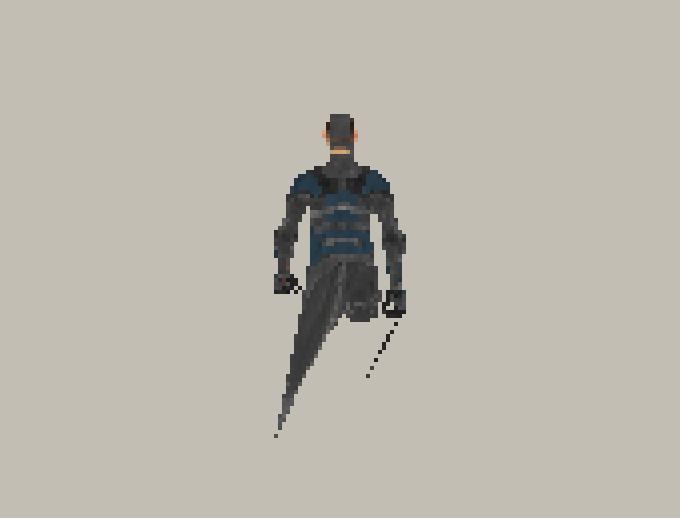
\includegraphics[width=0.45\textwidth]{Imagenes/E3/03_opengl_piernas_colapsadas.png}
    \caption{Primera carga de Exo Gray en OpenGL (acercamiento): la parte superior del cuerpo se anima correctamente, pero los vértices de las piernas se colapsan hacia el origen del modelo.}
    \label{fig:piernas_colapsadas}
\end{figure}

La pista estuvo en la forma del error: un vértice multiplicado por una matriz nula termina en el origen del modelo, que en un personaje de Mixamo está justo entre los pies. Al listar la armadura por índice encontramos que el exportador FBX de Blender escribe un \textit{cluster} por \emph{cada} hueso de la armadura, tenga pesos o no; con 112 huesos, los de las piernas (\texttt{LeftUpLeg} a \texttt{RightToeBase}) quedaban con los índices 102 a 110, fuera del arreglo \texttt{gBones[100]} del \textit{shader}. La parte superior funcionaba simplemente porque sus huesos aparecen antes en el árbol. La corrección fue borrar los 18 huesos sin pesos, todos hojas, con lo que la armadura bajó a 94 huesos y las piernas a índices menores que 100.

\textbf{Animación congelada.} En la misma prueba la consola reportó \texttt{Animation total frames: 249} para Exo Gray, cuando el clip de Mixamo tiene 32 cuadros. El exportador hornea la animación sobre el rango de la escena de Blender, que por omisión va de 1 a 250, así que el personaje daba un ciclo de caminata y se quedaba quieto en la última pose durante unos siete segundos antes de reiniciar. Se corrigió ajustando el rango de la escena al de la acción antes de exportar; después de eso la consola reporta 31 cuadros para los dos personajes.

\subsubsection{Pruebas exitosas}
Con las dos correcciones, Exo Gray se carga como una sola malla de 16\,738 vértices, con su textura completa, y camina sin deformaciones. Como comparación, el personaje de ejemplo tiene 2\,456 vértices y 68 huesos. La diferencia de tamaño sí se nota en un aspecto: \texttt{AnimatedModel} asigna los pesos recorriendo, para cada vértice, todos los pesos de todos los huesos, por lo que el tiempo de carga crece con el producto de ambos, y con Exo Gray el programa tarda alrededor de medio minuto en mostrar la escena.

\subsection{Experimentos de la Actividad 4: zona ampliada con casas, calles y banquetas}

\subsubsection{Objetivo del experimento}
La variación de esta actividad fue generar los alrededores a partir de las medidas de la ciudad en lugar de colocarlos a mano, para verificar que el mismo procedimiento se adapta a una ciudad de otro tamaño sin rehacer el modelado.

\subsubsection{Pruebas exitosas}
El guion se escribió primero sobre una versión preliminar de la ciudad que ocupaba $x \in [-2.2,\ 72]$ y $y \in [-20,\ 4]$, y con ella dejaba 7 casas por fila. Al cambiar al modelo definitivo de la Actividad 1, que es más angosto en $X$ y bastante más profundo en $Y$, no fue necesario tocar ninguna medida: el guion recalculó las manzanas a $79 \times 51$ unidades, bajó el número de casas a 6 por fila, ajustó la separación del segundo \textit{Array} de las casas a 89 unidades y la de las líneas de las avenidas a 63 unidades. Las casas, con sus puertas y ventanas, no cambiaron en absoluto, porque su modelado no depende del tamaño de la ciudad.

\subsubsection{Pruebas fallidas y análisis de errores}
En la primera ejecución en OpenGL la mayor parte de la ventana quedó cubierta por una superficie gris clara y el personaje no aparecía (Figura \ref{fig:camara_techo}). La cámara se había colocado a 6 unidades de altura y a $z = 50$, que en la ciudad ampliada cae justo sobre la fila de casas de enfrente; como el techo de las casas llega exactamente a 6 unidades, la cámara quedó dentro de uno de ellos. La corrección fue subirla a 10 unidades de altura e inclinarla $20^\circ$ hacia abajo, de modo que queda por encima de los techos y sigue viendo al personaje sobre la avenida.

\begin{figure}[H]
    \centering
    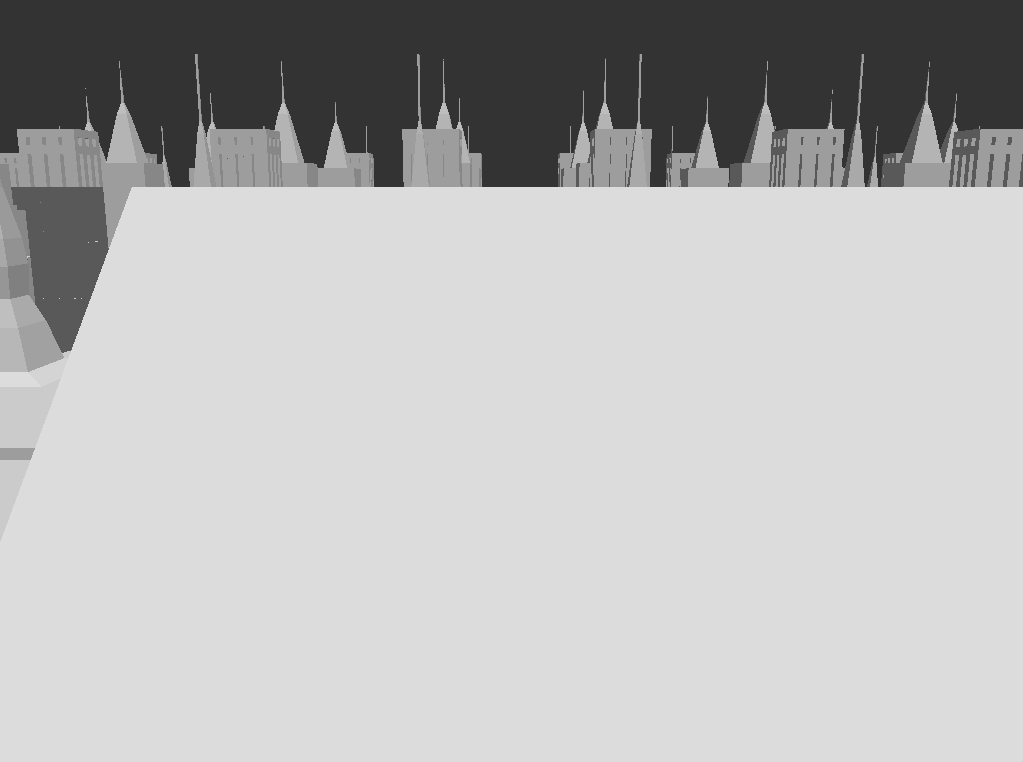
\includegraphics[width=0.6\textwidth]{Imagenes/E4/12_opengl_camara_dentro_techo.png}
    \caption{Primera ejecución de la zona ampliada en OpenGL: la cámara quedó dentro del techo de una casa de la fila de enfrente y el techo cubre casi toda la vista.}
    \label{fig:camara_techo}
\end{figure}
% ==============================================================================
% RESULTADOS
% ==============================================================================
% Instrucciones de la plantilla:
% - Por cada una de las actividades, describir detalladamente los resultados alcanzados, tanto de las solicitadas, como de los experimentos.
% - Incluir capturas de pantalla debidamente tituladas y referenciadas en el texto.
% - REGLA: No se aceptarán solo capturas de pantalla; deben estar explicadas.
% - Analizar ventajas y desventajas de la metodología aplicada.
% ==============================================================================

\section{Resultados}

A continuación se exponen y analizan los resultados obtenidos en cada una de las actividades prácticas y pruebas experimentales.

\subsection{Resultados de la Actividad 1}
En la Actividad 1 se logró la representación gráfica correcta de la escena interactiva. Como se observa en la Figura \ref{fig:resultado_act1}, el cauce de renderizado procesó satisfactoriamente las primitivas geométricas...

% Ejemplo de inserción de figura con título y referencia en el texto:
\begin{figure}[H]
    \centering
    % Coloca tu imagen en la carpeta Imagenes/ y descomenta la siguiente línea:
    % \includegraphics[width=0.75\textwidth]{Imagenes/resultado_actividad1.png}
    % Mientras tanto, un marco de demostración:
    \setlength{\fboxrule}{1pt}
    \framebox[0.75\textwidth]{\rule{0pt}{4cm}\large Captura de pantalla de la Actividad 1}
    \caption{Resultado visual obtenido al ejecutar la escena interactiva de la Actividad 1.}
    \label{fig:resultado_act1}
\end{figure}

\subsubsection{Análisis de ventajas y desventajas}
\begin{itemize}
    \item \textbf{Ventajas:} El enfoque utilizado mediante VAO/VBO optimiza la transferencia de memoria hacia la GPU, reduciendo la sobrecarga de la CPU por llamada de dibujo.
    \item \textbf{Desventajas:} Requiere un manejo explícito del ciclo de vida de los identificadores de recursos en memoria gráfica para prevenir fugas de memoria.
\end{itemize}

\subsection{Resultados de la Actividad 2}
% Describir resultados y capturas para la Actividad 2:
\textit{Describir detalladamente los resultados obtenidos en la segunda actividad y referenciar sus figuras correspondientes...}

\subsection{Resultados de la Actividad 3}
La adaptación en Blender dejó a Exo Gray como un modelo que \texttt{AnimatedModel} puede animar sin modificaciones: una malla, un material y 94 huesos. La Figura \ref{fig:atlas_exogray} muestra el atlas resultante, con el traje en la mitad izquierda y la cara y el cuerpo en la derecha, y la Figura \ref{fig:exogray_blender} muestra el modelo ya unido y animado dentro de Blender antes de exportarlo. Que la cara y el traje se vean en su lugar confirma que el recorrido de las coordenadas UV a cada mitad del atlas fue correcto.

\begin{figure}[H]
    \centering
    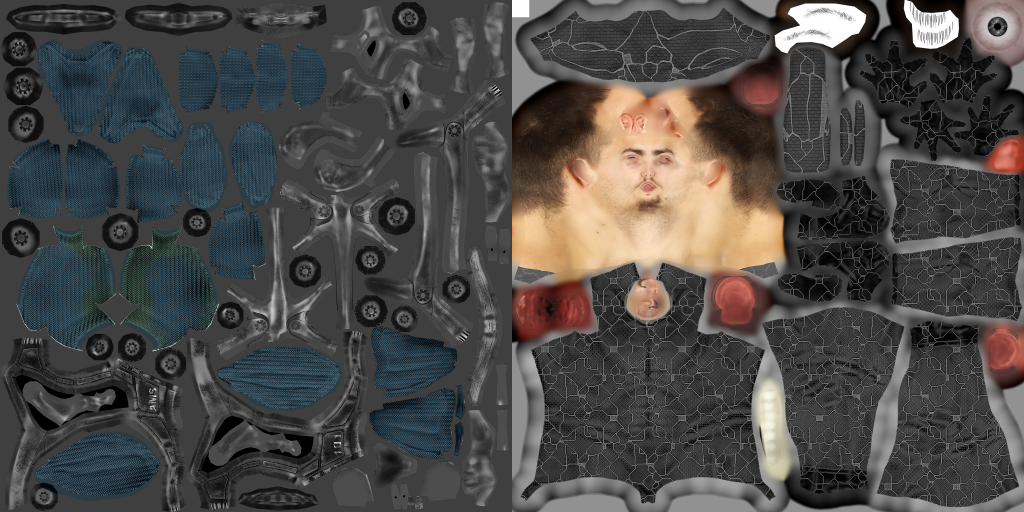
\includegraphics[width=0.75\textwidth]{Imagenes/E3/01_exogray_atlas_texturas.png}
    \caption{Atlas de $4096 \times 2048$ píxeles generado por \texttt{personaje\_act3.py}: a la izquierda la textura del traje y a la derecha la de la cara y el cuerpo.}
    \label{fig:atlas_exogray}
\end{figure}

\begin{figure}[H]
    \centering
    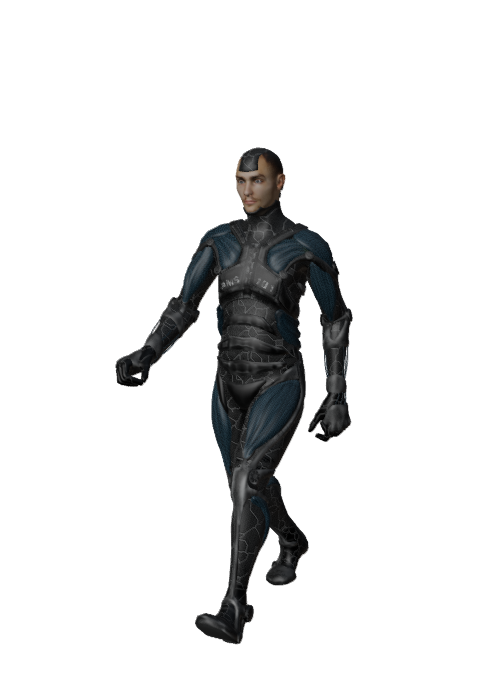
\includegraphics[width=0.32\textwidth]{Imagenes/E3/02_exogray_blender_una_malla.png}
    \caption{Exo Gray en Blender después de la adaptación: una sola malla de 16\,738 vértices con el atlas aplicado, a mitad del ciclo de caminata.}
    \label{fig:exogray_blender}
\end{figure}

En OpenGL el personaje aparece sobre la avenida de enfrente de la ciudad y responde a las cuatro flechas (Figura \ref{fig:exogray_opengl}): las flechas \texttt{Arriba} y \texttt{Abajo} lo desplazan en la dirección hacia la que mira y las laterales lo giran sobre el eje $Y$, mientras la caminata se reproduce en su lugar. Con la tecla \texttt{G} se cambia al personaje de ejemplo del laboratorio (Figura \ref{fig:personaje_clase}), que se mueve con exactamente los mismos controles. Como los dos personajes comparten la posición y la orientación, el cambio ocurre en el mismo punto de la escena.

\begin{figure}[H]
    \centering
    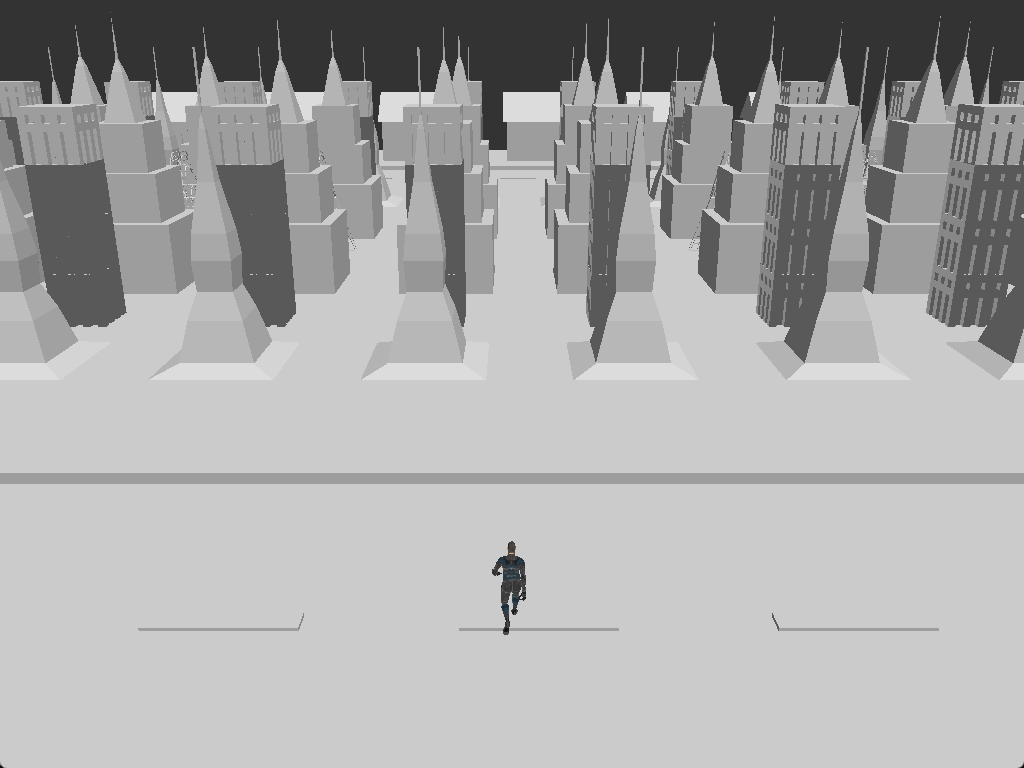
\includegraphics[width=0.75\textwidth]{Imagenes/E3/04_opengl_exogray_ciudad.png}
    \caption{Exo Gray cargado en OpenGL con \texttt{AnimatedModel}, sobre la avenida de enfrente de la ciudad.}
    \label{fig:exogray_opengl}
\end{figure}

\begin{figure}[H]
    \centering
    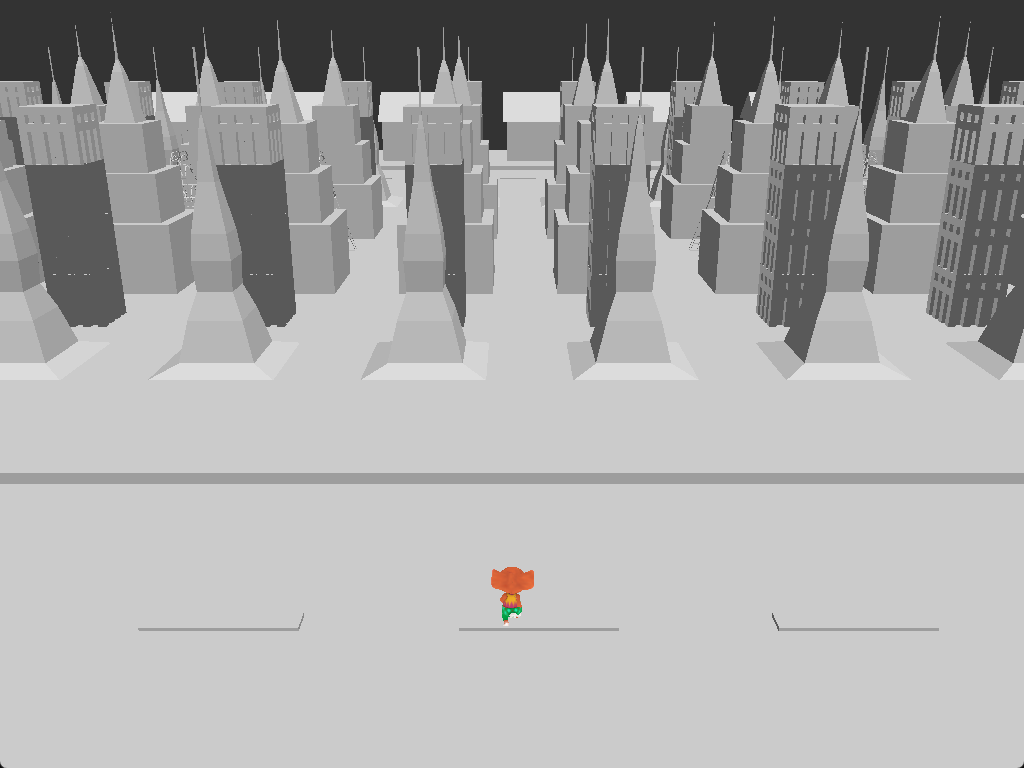
\includegraphics[width=0.75\textwidth]{Imagenes/E3/05_opengl_personaje_clase.png}
    \caption{El personaje de ejemplo del laboratorio (\texttt{character.fbx}) en la misma posición, después de presionar la tecla \texttt{G}.}
    \label{fig:personaje_clase}
\end{figure}

\subsubsection{Análisis de ventajas y desventajas}
\begin{itemize}
    \item \textbf{Ventajas:} Adaptar el modelo en lugar del cargador deja intacta la clase que usan las demás prácticas, y como todo el proceso quedó en un guion, cualquier otro personaje de Mixamo se puede preparar con el mismo procedimiento cambiando solo el archivo de entrada.
    \item \textbf{Desventajas:} El atlas pesa 12 MB y, al juntar las texturas en una sola, cada parte del cuerpo dispone de la mitad de la resolución horizontal que tenía. Además, el tiempo de carga crece mucho con el número de vértices por la forma en que la clase asigna los pesos.
\end{itemize}

\subsection{Resultados de la Actividad 4}
La secuencia del modelado quedó registrada en Blender paso a paso. La Figura \ref{fig:casa_pasos} resume la construcción de la casa: los muros subdivididos en tres columnas, las puertas y ventanas hundidas con \textit{Inset} y \textit{Extrude}, y el techo de dos aguas obtenido al escalar a cero la cara superior de un cubo.

\begin{figure}[H]
    \centering
    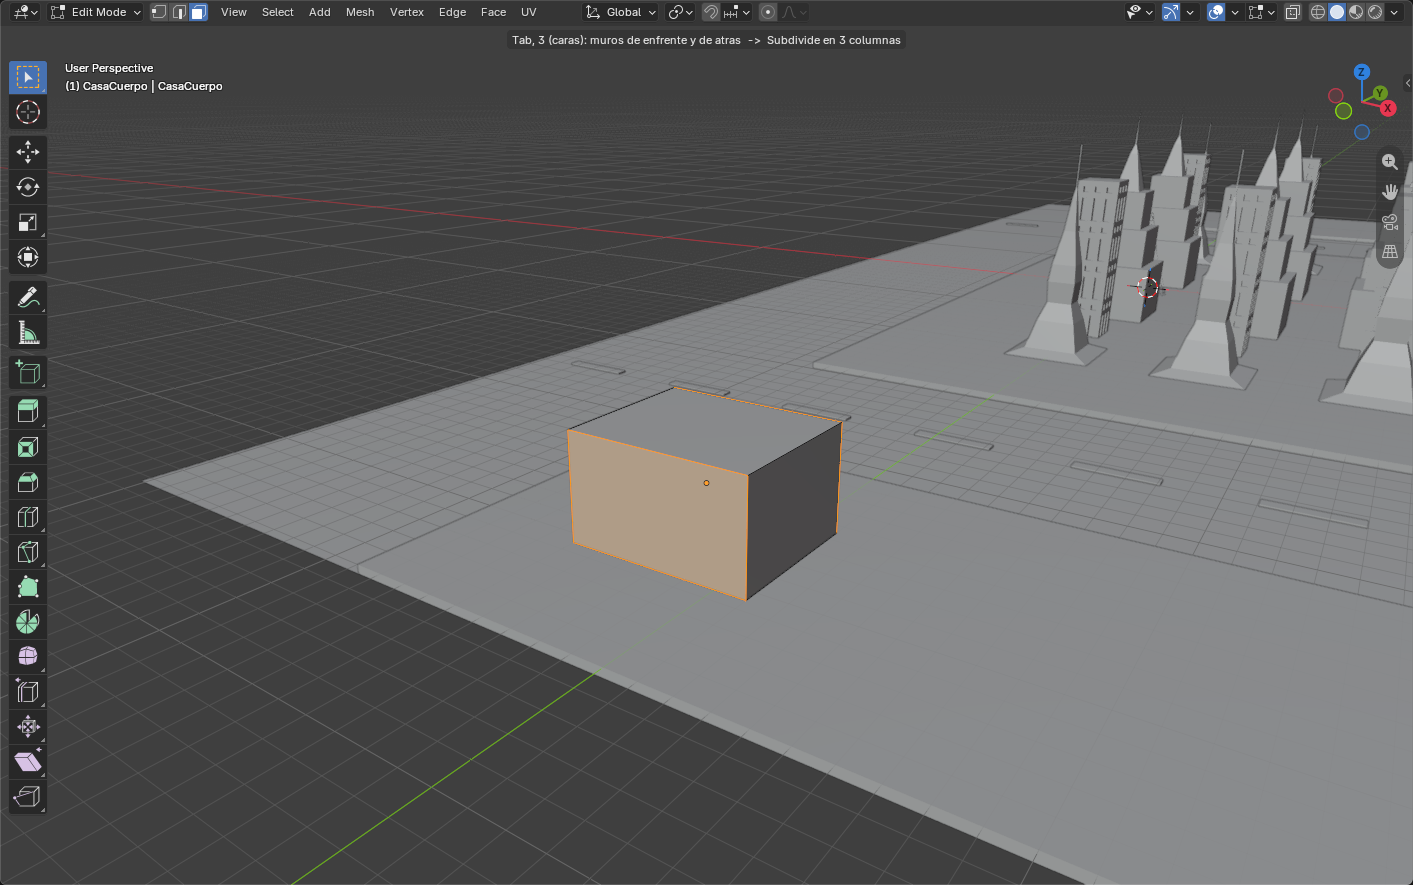
\includegraphics[width=0.32\textwidth]{Imagenes/E4/06_casa_subdivide.png}
    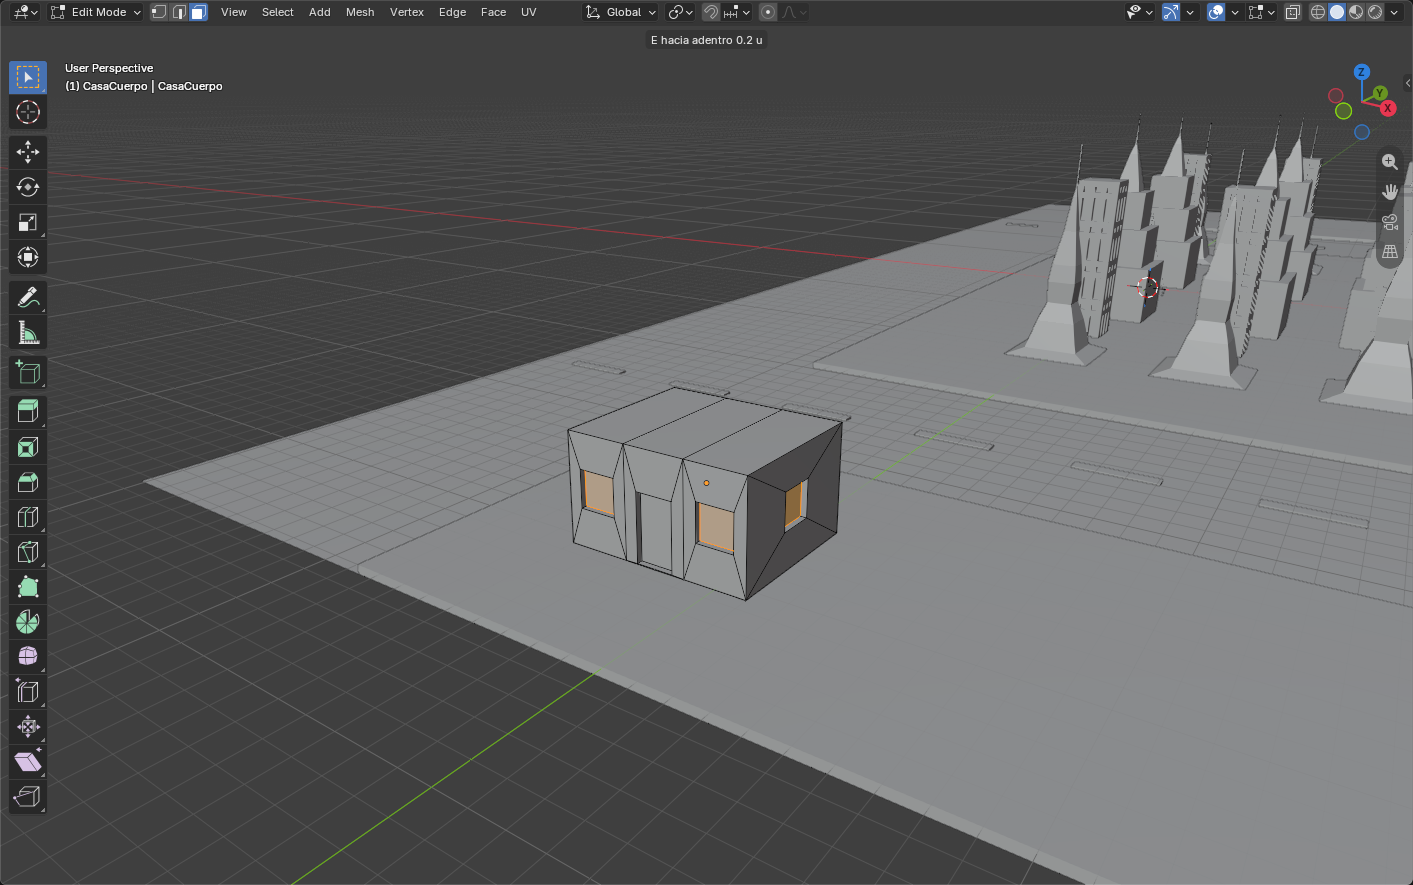
\includegraphics[width=0.32\textwidth]{Imagenes/E4/08_casa_ventanas.png}
    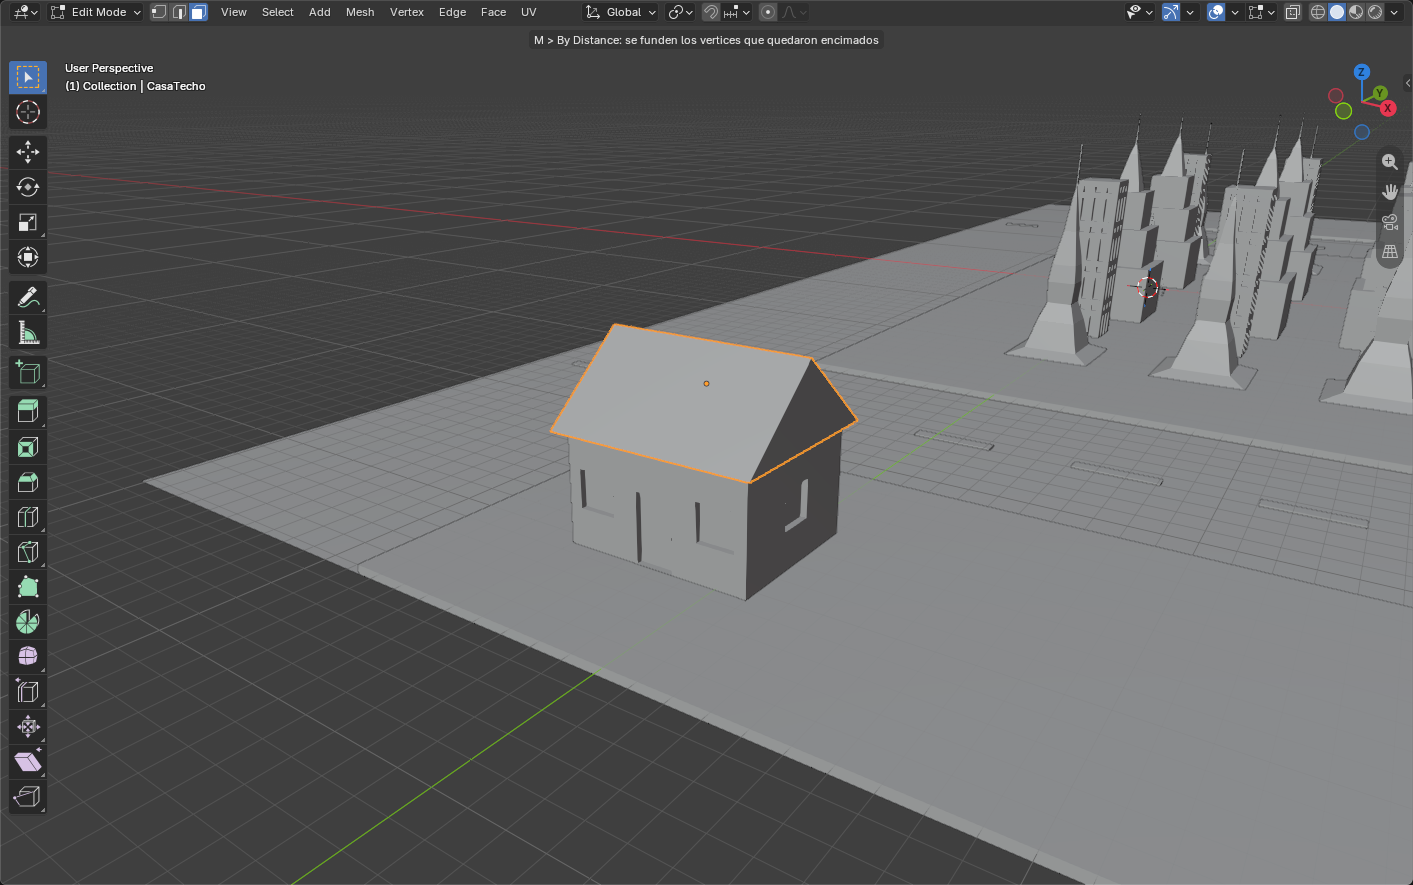
\includegraphics[width=0.32\textwidth]{Imagenes/E4/09_casa_techo_dos_aguas.png}
    \caption{Construcción de la casa: subdivisión de los muros en tres columnas (izquierda), puertas y ventanas hundidas (centro) y techo de dos aguas con \textit{S Y 0} (derecha).}
    \label{fig:casa_pasos}
\end{figure}

La Figura \ref{fig:zona_ampliada} muestra el modelo completo antes de exportarlo: la ciudad de la Actividad 1 sobre su banqueta, las dos avenidas con sus líneas centrales y las dos filas de seis casas, cada una con la puerta hacia su avenida. El archivo exportado, \texttt{Ciudad.fbx}, pesa 6.3 MB.

\begin{figure}[H]
    \centering
    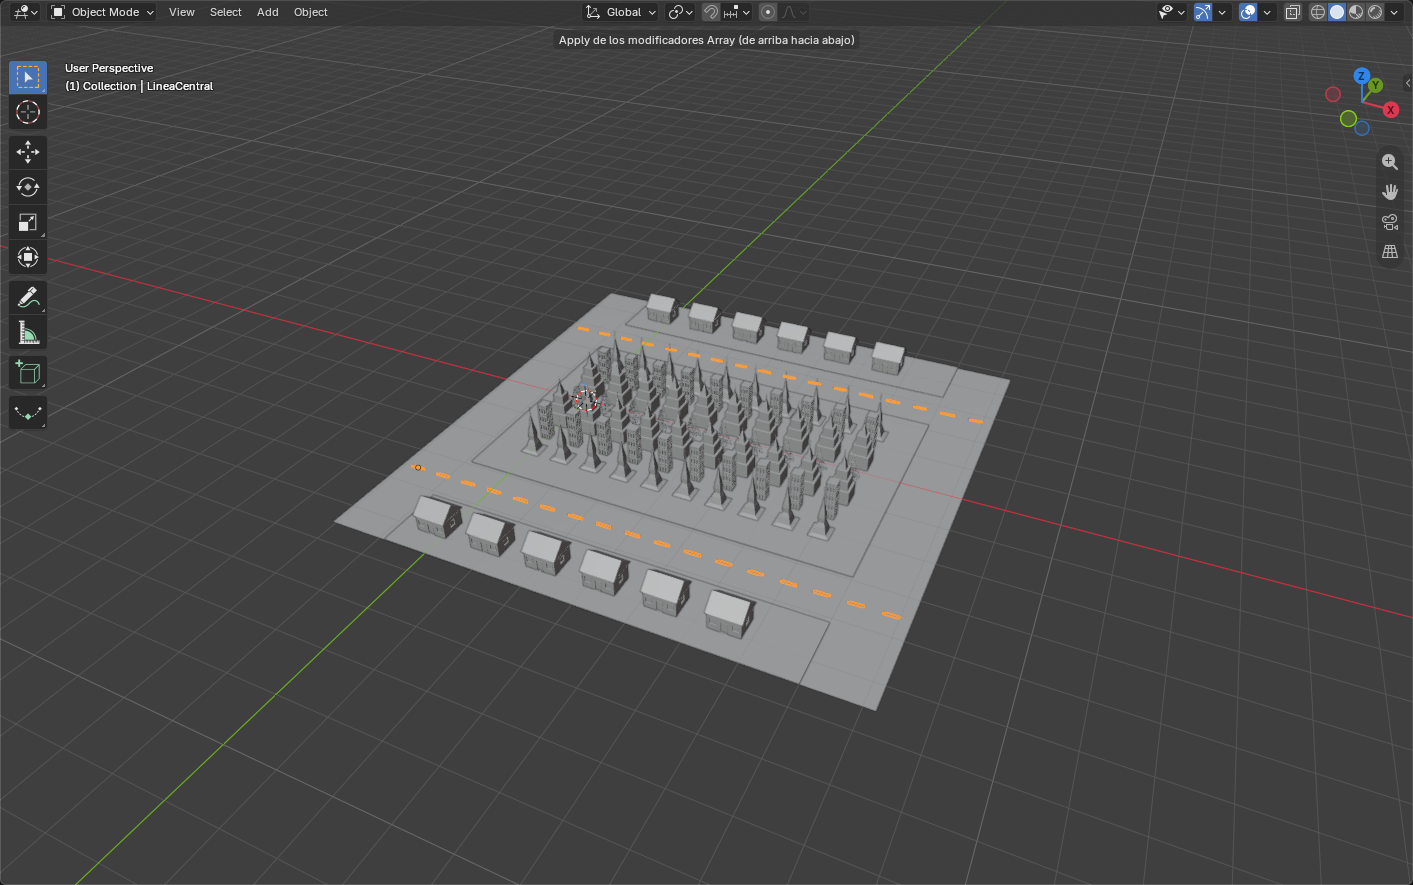
\includegraphics[width=0.8\textwidth]{Imagenes/E4/11_zona_ampliada.png}
    \caption{Zona ampliada en Blender: manzana central con los edificios, avenidas de enfrente y de atrás con sus líneas centrales y dos filas de casas.}
    \label{fig:zona_ampliada}
\end{figure}

Cargado en OpenGL, el modelo se ve completo desde la avenida (Figura \ref{fig:ciudad_opengl}). Sin usar colores, la diferencia de altura entre banqueta y asfalto y la luz direccional del \textit{shader} gris bastan para distinguir la calle, el borde de la banqueta y las caras de cada edificio. Al recorrer la escena con el personaje, la avenida y las calles laterales permiten rodear toda la manzana de los edificios.

\begin{figure}[H]
    \centering
    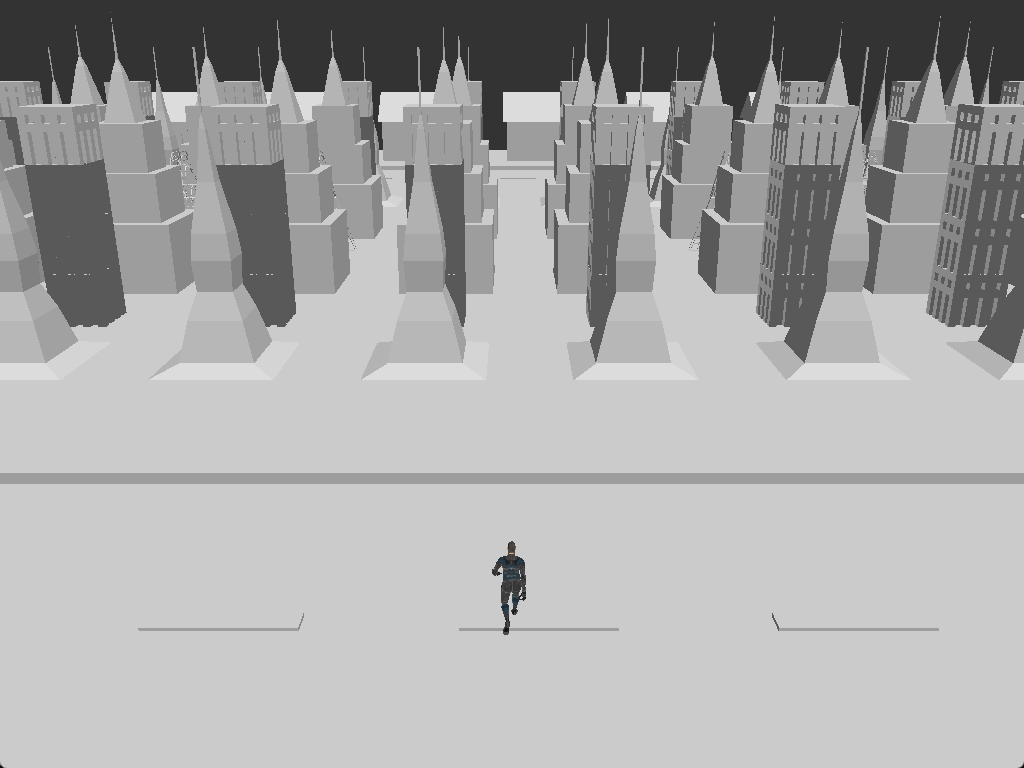
\includegraphics[width=0.75\textwidth]{Imagenes/E4/13_opengl_ciudad_ampliada.png}
    \caption{Ciudad.fbx en OpenGL con el \textit{shader} gris, vista desde la avenida de enfrente.}
    \label{fig:ciudad_opengl}
\end{figure}

\subsubsection{Análisis de ventajas y desventajas}
\begin{itemize}
    \item \textbf{Ventajas:} Al calcular el trazo desde la caja de la ciudad, el procedimiento se adaptó sin cambios a un modelo de otro tamaño, y el uso de \textit{Array} hace que agregar o quitar casas sea cuestión de cambiar un solo número.
    \item \textbf{Desventajas:} Como todo se exporta en un solo FBX con un solo material, en OpenGL la ciudad, las casas y las calles comparten el mismo \textit{shader} y no pueden tratarse por separado; además, las casas son copias idénticas, así que la zona se ve repetitiva.
\end{itemize}
% ==============================================================================
% CONCLUSIONES INDIVIDUALES
% ==============================================================================
% Instrucciones de la plantilla:
% Formato: #CUENTA: CONCLUSIÓN
% Cada integrante del equipo debe redactar de forma personal, concreta y coherente sus conclusiones individuales sobre la práctica y los conceptos gráficos aprendidos.
% ==============================================================================

\section{Conclusiones Individuales}

\subsection*{\#321137135: Basilio Illescas Andrés}
% Redactar la conclusión individual del alumno aquí:
A través de las actividades implementadas, se logró afianzar el conocimiento sobre...

\subsection*{\#424065465: Cruz Macedo Samuel Santiago}
% Redactar la conclusión individual del alumno aquí:
El análisis de los experimentos realizados permitió identificar...

\subsection*{\#321258173: Medel Piña Ángel de Jesús}
% Redactar la conclusión individual del alumno aquí:
La práctica permitió contrastar la teoría vista en clase con la implementación en OpenGL...

\subsection*{\#321150503: Pérez Olvera Alexis Abraham}
% Redactar la conclusión individual del alumno aquí:
Durante el desarrollo de la práctica se comprendieron los conceptos fundamentales de...

\subsection*{\#320224159: Segura Cedeño Luisa María}
% Redactar la conclusión individual del alumno aquí:
Como resultado del desarrollo de los algoritmos y pruebas gráficas...

% ==============================================================================
% ENLACE AL VIDEO
% ==============================================================================
% Instrucciones de la plantilla:
% Incluir un video de 5 a 10 minutos de duración, donde se explique un compendio de los resultados alcanzados por cada una de las actividades. Un solo video. 
% Verificar que el video esté disponible para su revisión y no tenga restricciones de acceso.
% ==============================================================================

\section{Enlace al Video Demostrativo}

A continuación se proporciona el enlace al video demostrativo de la práctica (con una duración de entre 5 y 10 minutos), en el cual se expone de forma detallada el funcionamiento, compilación y compendio de resultados de cada una de las actividades realizadas:

\vspace{0.4cm}
\begin{center}
    \renewcommand{\arraystretch}{1.5}
    \begin{tabular}{|>{\centering\arraybackslash}p{0.85\textwidth}|}
        \hline
        \textbf{Enlace oficial de la demostración:} \tabularnewline
        \url{\enlaceVideo} \tabularnewline
        \footnotesize\textit{(Asegurarse de que el video esté disponible para revisión y sin restricciones de acceso)} \tabularnewline
        \hline
    \end{tabular}
\end{center}
\vspace{0.4cm}

% ==============================================================================
% REFERENCIAS BIBLIOGRÁFICAS (FORMATO APA)
% ==============================================================================
% Instrucciones de la plantilla:
% - Lista de fuentes de información en formato APA.
% - IMPORTANTE: Enlistar preferentemente libros, revistas, capítulos.
% - Si se citan sitios web, hacerlo conforme al estilo APA.
% ==============================================================================

\renewcommand{\refname}{Referencias Bibliográficas}
\begin{thebibliography}{99}

\bibitem{hearn_baker}
Hearn, D., Baker, M. P., \& Carithers, W. (2011). \textit{Computer Graphics with OpenGL} (4.ª ed.). Pearson Prentice Hall.

\bibitem{foley}
Foley, J. D., Van Dam, A., Feiner, S. K., \& Hughes, J. F. (1996). \textit{Computer Graphics: Principles and Practice in C} (2.ª ed.). Addison-Wesley Professional.

\bibitem{learnopengl}
de Vries, J. (2020). \textit{Learn OpenGL: Learn modern OpenGL graphics programming in a step-by-step fashion}. Recuperado de \url{https://learnopengl.com/}

\bibitem{khronos_opengl}
Khronos Group. (s.f.). \textit{OpenGL 3.3 Reference Pages}. The Khronos Group Inc. Recuperado de \url{https://registry.khronos.org/OpenGL-Refpages/}

\bibitem{teodoro_vite}
Teodoro-Vite, S., et al. (2019). \textit{Fundamentos y Técnicas del Cómputo Gráfico}. Facultad de Ingeniería, Universidad Nacional Autónoma de México.

\end{thebibliography}


\end{document}
